\documentclass[../masterarbeit.tex]{subfiles}
\begin{document}
	




\subsection{Model training and evaluation}
In this chapter, the training phase and the evaluation of the three machine learning classification models Logistic Regression, Linear Discriminant Analysis and Support Vector Machine are explained. The structure of the models and their evaluation will be discussed in more detail. The three machine learning models are trained and evaluated in the order Logistic Regression, Linear Discriminants Analysis. The three models were trained on the respective data sets optimized for the models, wich are described before in section 4.2.2. A confusion matrix was created for every model as well as cross-validated accuracy, precision and recall metric. In addition, cross validated ROC curves were created for the Logistic Regression, LDA and SVM models. Before training and evaluating the algorithms on the optimized sets, the datasets were standardized with the StandardScaler \textcite[]{Sklearn_StandardScaler:2022} function mentioned in section 3.1 about data preprocessing.  \\~\\



The training and evaluation phase of the Logistic Regression model is described as the first of the three classification models. The Logistic Regression model from the Sklearn.linear\_model library \textcite[]{Scikit-learn-logistic-regression:2022} was trained with its default parameters. \\
\begin{figure}[h]
    \centering
    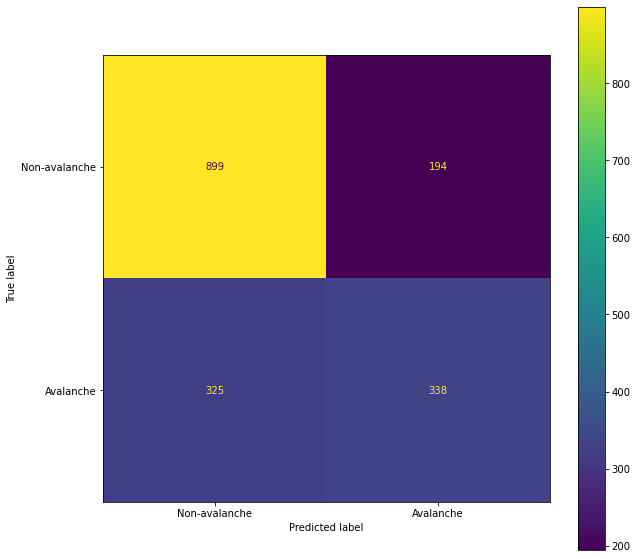
\includegraphics[scale=0.5]{confusion_matrix_LR.png}
    \source{created by the author}
    \caption{The confusion matrix for the Logistic Regression model.}
\end{figure}
In order to gain a direct insight into the predictions of the machine learning model, the confusion matrix, wich is shown in figure 18, was created for the model in the course of the study. The confusion matrix represents the four output types of the binary classification model as mentioned in chapter 3.4. In the case of this study the binary states are "Avalanche" and "Non-avalanche". The confusion matrix in figure 18 presents the predicted states on the Y-axis and the true states on the X-axis. For the creation of the confusion matrix the train test split function from the Python library sklearn.model\_selection \textcite[]{Scikit-learn-train-test-split:2022} was performed on the data set with a train test ratio of 75\% training set to 25\% validation set. So in total 5263 training samples and 1758 test samples are used. To create the confusion matrix, the plot function ConfusionMatrixDisplay \textcite[]{Scikit-learn-confusion-matrix:2022} from the library Sklearn.metrics is used. In the top left corner of the matrix the 899 True Negative predicted Non-avalanches are represented. 194 actual Non-avalanches were predicted as Avalanches shown in the top right quarter of the matrix. The Logistic Regression Model also predicted 325 Avalanches as Non-avalanches and 338 actual Avalanche samples as Avalanches. So the total number of samples falsely predicted by the Logistic Regression model is 519. The total number of correctly predicted samples is 1239. The number of Avalanche samples included in the test set is 663 and the number of Non-avalanche samples is 1093. As the confusion matrix shows, the percentage of correctly determined avalanches is smaller compared to the percentage of correctly determined non-avalanche samples. This could indicate a bias toward the non-avalanche samples caused by the fact that the dataset includes more Non-avalanche samples than Avalanche samples, as mentioned in chapter 4.1.5. \\~\\
\begin{figure}[h]
    \centering
    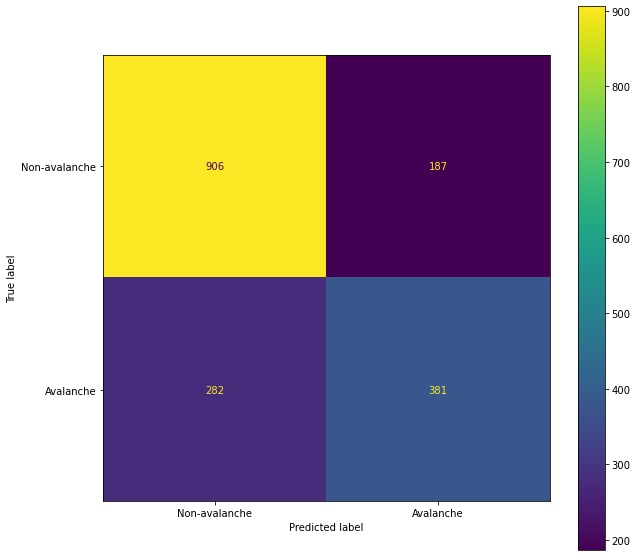
\includegraphics[scale=0.5]{confusion_matrix_LDA.png}
    \source{created by the author}
    \caption{The confusion matrix for the Linear Discriminant Analysis model.}
\end{figure}
The second model trained and evaluated is the Linear Discriminant Analysis model.
For this task, the LDA model from the sklearn.discriminant\_analysis \textcite[]{Scikit-learn-lda:2022} is used. The model was also trained on with the default parameters defined by the library. For all following training and evaluation processes of the model, the data set optimized for the LDA by the genetic algorithm, which is listed in Table 7, was used. \\
The confusion matrix represented in figure 19 shows was created for the purpose of getting an overview over the predictions made by the Linear Discriminant Analysis model. The confusion matrix was created with the same function as that one for the Logistic Regression model, as well as the 75\% to 25\% split for the train and validation dataset. The number of Non-avalanche samples of the test set is 1093 and the number of Avalanches 663, wich are exactly the same numbers as for the Logistic Regression model.
The number of True-Positive predicted samples shown in that confusion matrix is 381. The sum of Avalanche samples wich were predicted as Non-avalanche ones is 282. Furthermore, the number of non-avalanche samples predicted by the Linear Discriminant Analysis model True-Negative is 906. In the upper right quarter of the confusion matrix, the incorrectly predicted non-avalanches are plotted, with the number of False-Positive values at 194. As can be seen the number of True-Positive predicted samples is larger  and the number True-Negative predicted samples is similar compared to the predictions of the Logistic Regression model. It is especially with the prediction of the avalanche samples further away from coincidence. This indicates that there may be sufficient information in the data to predict snow avalanches for topographically defined mountain slopes. In total 1287 samples have been predicted correctly by the LDA model. The number is slightly higher than that one of the Logistic Regression, because the LDA predicted more Avalanche samples correctly.\\~\\
\begin{figure}[h]
    \centering
    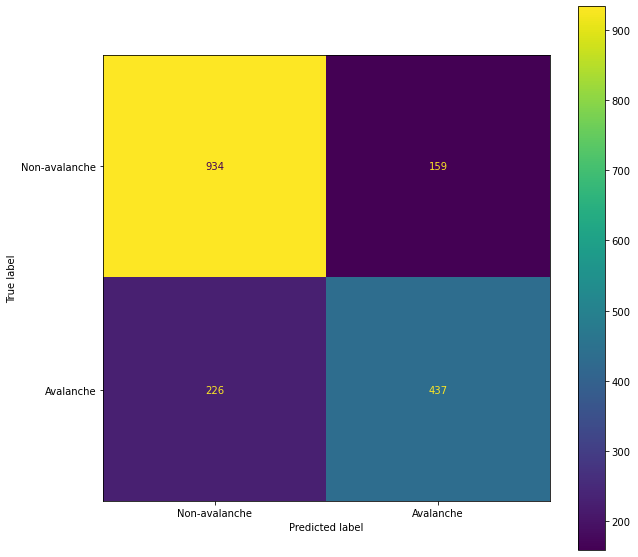
\includegraphics[scale=0.5]{confusion_matrix_SVM.png}
    \source{created by the author}
    \caption{The confusion matrix for the Support Vector Machine model.}
\end{figure}
The Support Vector Machine is the last model trained for the study of this thesis. The SVM implementation used is the C-Support Vector Classification (SVC) \textcite[]{Scikit-learn-svc:2022} from the Sklearn.svm library. The parameters used for the model are also the default values from the documentation. \\
Also in the case of the SVM model, the confusion matrix was created using a 75\% to 25\% train test ratio of the data. In addition, the number of avalanche and non-avalanche samples in the training and test set is the same as in the previous two models. The first thing to notice when looking at the confusion matrix in Figure 20, which was created using the SVM model, is the color difference between the correctly and incorrectly predicted samples. The value of the correctly predicted avalanche samples is the highest of the three models at 437, which makes the square stand out more from the one to the left, which represents the false negative predicted values, than in the confusion matrix for the logistic regression model. The number of False-Negative predicted values shown in the bottom left corner of the confusion matrix is 226, wich is 99 samples less than with the Logistic Regression model and 56 less then the LDA. The present difference between correctly and incorrectly predicted avalanche samples suggests that the predictions are not coincidental and that the data contain information for the prediction of avalanches. The sum of samples predicted as True-Negative is 934. In addition, 159 non-avalanche samples were predicted to be avalanches. In total, 1371 samples have been predicted correctly by the SVM model. So it predicted more samples correctly than the LDA and the Logistic Regression models. The model also predicted 385 samples incorrectly wich are 84 samples less than the LDA model. \\~\\













To gain more information about the quality of the predictions, made by the three machine learning models, a 10-fold cross-validation was performed on each of the models and a series of the evaluation metrics accuracy, recall and precision were created in conjunction with them. As explained in chapter 3.4.5, cross-validation offers the possibility to perform an extensive validation over the whole dataset and at the same time to use a large part of the dataset for the training of the machine learning models at each iteration. So the resulting metrics are more representative for the quality of the predictions than the 75\% to 25\% train test split made for the confusion matrices before. For each of the resulting metrics, the maximum, minimum, and average values that occurred during the 10-fold cross-validation are represented in table 8. The first score wich is represented in table 8 is the accuracy score. As mentioned in section 3.4.1, the accuracy score represents the total number of correctly predicted samples compared to the total number of samples. The average accuracy score is 0.735 for the Logistic Regression model, 0.732 for the LDA model and 0.754 for the SVM model. So the values are similar for all three models, but that one of the SVM is higher than the others. The maximum accuracy is 0.806 for the Logistic Regression, 0.800 for the LDA and 0.803 for the SVM. In this case the values of all three models are similar to each other. The values of the minimum accuracy in the same order as before are 0.678, 0.690, 0.713. As can be seen, the SVM has the highest minimum accuracy, the LDA follows and last is the Logistic Regression. Causing the fact that there are less Avalanche samples included in the datasets than Non-avalanches, the balanced accuracy score is also calculated for the three models. The average balanced accuracy score is 0.705 for the Logistic Regression model. This value is 0.030 smaller than the normal accuracy score for this model. For the Linear Discriminant Analysis model the balanced accuracy score is 0.700, wich is 0.032 smaller than the average accuracy score for the same model. The value of the average balanced accuracy for the SVM model is 0.724, wich is the highest value of the three. Similar to the balanced accuracy score of the two models Logistic Regression and LDA it is about 0.030 smaller than the accuracy score for the model. As already mentioned in chapter 3.4.1 about the accuracy score, the value of the balanced accuracy score is often smaller than that one of the accuracy score in the case of an unbalanced data set. In contrast to the most previous metric values, the value of the maximum balanced accuracy score for the Logistic Regression model is the largest of the three models at 0.788. The value for the LDA is 0.765 and for the SVM 0.779. However, the value of the minimum balanced accuracy score for the Logistic Regression model is also the lowest with 0.636 compared to 0.659 and 0.663 for the LDA and SVM. \\~\\
\begin{table}[!ht]
    \centering
    \begin{tabular}{|l|l|l|l|}
    \hline
         & Logistic Regression & LDA & SVM \\ \hline
        Average accuracy & 0.735356 & 0.732791 & 0.754446 \\ \hline
        Max accuracy & 0.806268 & 0.800853 & 0.803419 \\ \hline
        Min accuracy & 0.678063 & 0.690883 & 0.713675 \\ \hline
        Average balanced accuracy & 0.705463 & 0.700595 & 0.724890 \\ \hline
        Max balanced accuracy & 0.788748 & 0.765140 & 0.779399 \\ \hline
        Min balanced accuracy & 0.636473 & 0.659482 & 0.663706 \\ \hline
        Average precision & 0.692394 & 0.693510 & 0.720818 \\ \hline
        Max precision & 0.831579 & 0.825000 & 0.809278 \\ \hline
        Min precision & 0.570571 & 0.587859 & 0.613636 \\ \hline
        Average recall & 0.577125 & 0.562296 & 0.597944 \\ \hline
        Max recall & 0.755556 & 0.703704 & 0.762963 \\ \hline
        Min recall & 0.379182 & 0.425926 & 0.449814 \\ \hline
    \end{tabular}
    \caption{A tabular arrangement showing the results of training the machine learning models and evaluating them using the metrics Accuracy, Precision and Recall in the course of 10-fold cross-validations.}
\end{table}
Another evaluation metric calculated in this evaluation process and represented in table 8 is the precision score. The value of the average precision score over the 10-fold cross-validation, calculated for the Logistic Regression model, is 0.692. For the LDA the average of the score is 0.693, wich is similar to the Logistic Regression model. The SVM has the highest average precision score of 0.720 over the ten iterations of cross validation. The metric evaluates the proportion of positively predicted samples that are actually positive. The Logistic Regression model had both the highest maximum precision score of 0.831 and the lowest minimum precision score of 0.570 of the three models. The next lower maximum precision score of 0.825 and the following minimum precision score of 0.587. The SVM has the lowest maximum precision score of 0.809 and the highest minimum precision score of 0.613. As can be seen in the table, the maximum precision score of the SVM is lower than that of the other models, but the average value over the 10 iterations is higher than the scores of the other models. The last metric calculated in the course of the evaluation of the three machine learning models and shown in table 8 is the recall score. The score in the context of this work refers only to the avalanches and the proportion of avalanches that were correctly predicted. The value of the Logistic Regression models average recall is 0.577. For the LDA model the value of the score is 0.562 and for the SVM model it is 0.597. As can be seen all values are smaller than the average values of the other scores. But also all of these values are above chance. The minimum and maximum values of the recall in the cross validation of the three models drift from each other. Thus, the minimum value of the recall of the Logistic Regression model is 0.379, which is smaller than chance, which is 0.5, and the maximum value of 0.755 is similar to the average accuracy score and 0.376 larger than the minimum and thus almost twice as large. Also the LDAs maximum recall value is about 0.703 an its minimum is 0.425. Recently, the maximum and minimum recall values of the SVM model are also different with 0.762 and 0.449. While all of the maximum and average recall score values are above the chance value of 0.5, the three minimum values are all below the value. \\~\\

After that step the last evaluation step made in case of this study, are ROC-curves in combination with the Area under the curve (AUC) score. For the three machine learning models the ROC curve and AUC score is calculated during 10-fold cross-validations, to obtain representative validation values. The graphs represented in the figures 21, 22 and 23 do all show a red striped straight line from \((0,0)\) to \((1,1)\). This line represents chance. So if the ROC-curve of a model is near to that line it is near to chance. Also if the values are below the chance, the model might have a false interpretation of the input data. A description of the ROC-curve and AUC value can be found in chapter 3.4.4.





In addition, three more ROC curves and AUC values were calculated for the three machine learning models without the use of 10-fold cross-validation and visualized in a fourth plot. These curves can be seen in Figure 24.






\begin{figure}[h]
    \centering
    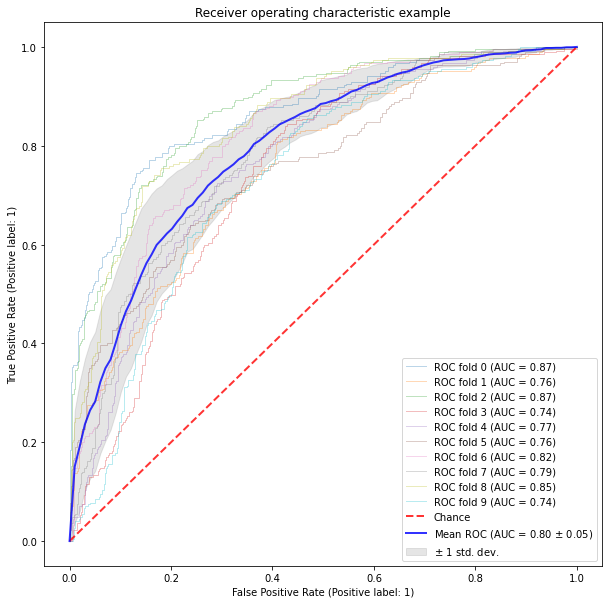
\includegraphics[scale=0.5]{ROC_AUC_LR.png}
    \source{created by the author}
    \caption{The ROC curve with AUC statistics with 10-fold cross-validation for the Logistic Regression model.}
\end{figure}




\begin{figure}[h]
    \centering
    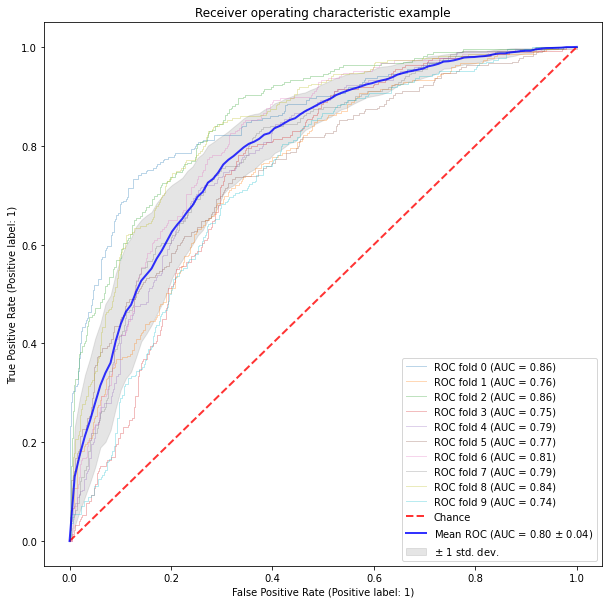
\includegraphics[scale=0.5]{ROC_AUC_LDA.png}
    \source{created by the author}
    \caption{The ROC curve with AUC statistics with 10-fold cross-validation for the LDA model.}
\end{figure}


The standard linear SVM is a discrete classifier so in terms of a roc curve it would just be a point.
The "RBF" kernel used as default for the SVC Implementation from Sklearn makes it possible to have a threshold and so also to get a ROC curve. For this study the SVC implementation is used with the default kernel "RBF". 


\begin{figure}[h]
    \centering
    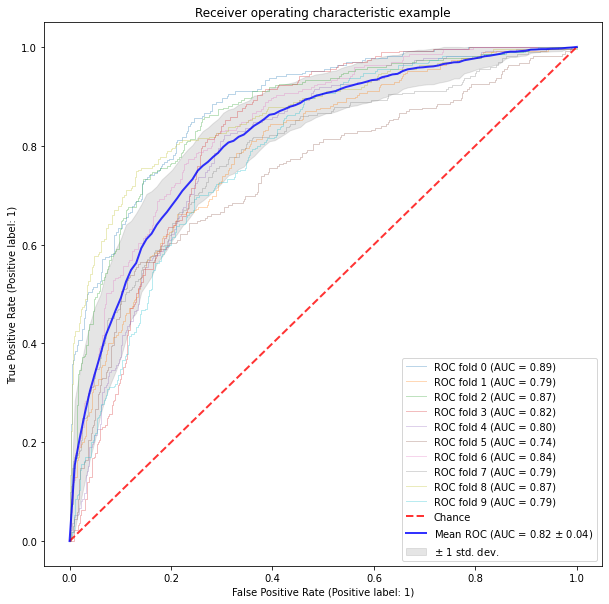
\includegraphics[scale=0.5]{ROC_AUC_SVM.png}
    \source{created by the author}
    \caption{The ROC curve with AUC statistics with 10-fold cross-validation for the SVM model.}
\end{figure}





\begin{figure}[h]
    \centering
    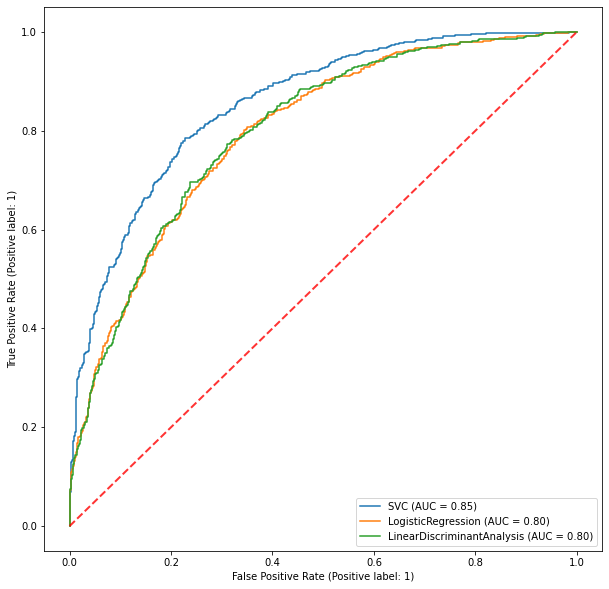
\includegraphics[scale=0.5]{ROC_AUC_Comparison.png}
    \source{created by the author}
    \caption{A comparison of the ROC curve and AUC statistic for the Logistic Regression, LDA and SVM models.}
\end{figure}

\end{document} 